\documentclass{if-beamer}

% --------------------------------------------------- %
%                  Presentation info	              %
% --------------------------------------------------- %
\title[Lecture 3]{Lecture 3}
\subtitle{Computer Hardware and The Unix Operating System}
\author{Instructor: Ashley Gannon}
\date{ISC3313 Fall 2021}
\logo{

\includegraphics[scale=0.08]{figures/FSULogo.png}
}
\subject{Presentation subject} % metadata

\graphicspath{{figures/}}
% --------------------------------------------------- %
%                    Title + Schedule                 %
% --------------------------------------------------- %
\begin{document}

\begin{frame}
  \titlepage
\end{frame}
% --------------------------------------------------- %
%                      Presentation                   %
% --------------------------------------------------- %
\begin{frame}
	\frametitle{Von Neumann Architecture}
	\begin{figure}
		\centering
		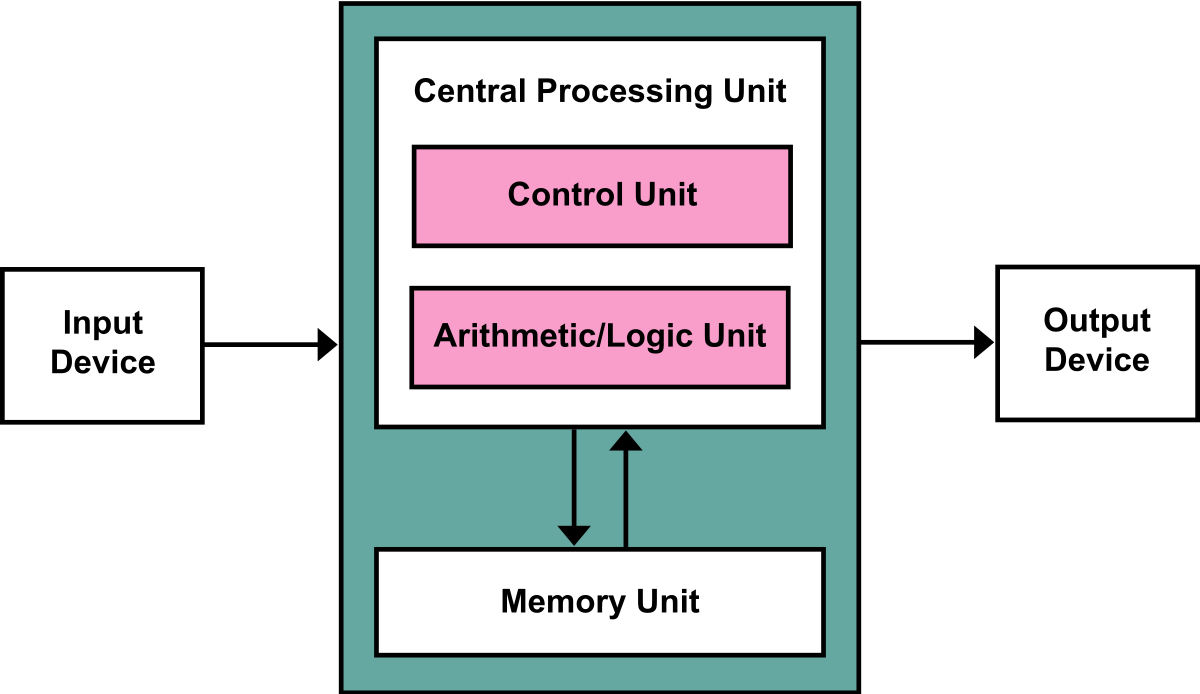
\includegraphics{figures/vonNeumannArch.png}
	\end{figure}
\end{frame}
\section{Components}
\begin{frame}
\frametitle{Memory Cell}
\begin{itemize}
	\item The fundamental unit of computer memory is a memory cell.
	\item This is an electronic circuit that stores one binary digit (\textit{bit} for short) of information.
	\item This bit represents a logical state with one of two factors - 0 or 1, on or off, high or low voltage.
	\item The value of a bit is stored until it is changed by the set/reset process, and can be accessed by reading the memory cell.
\end{itemize}

\begin{figure}
	\center
	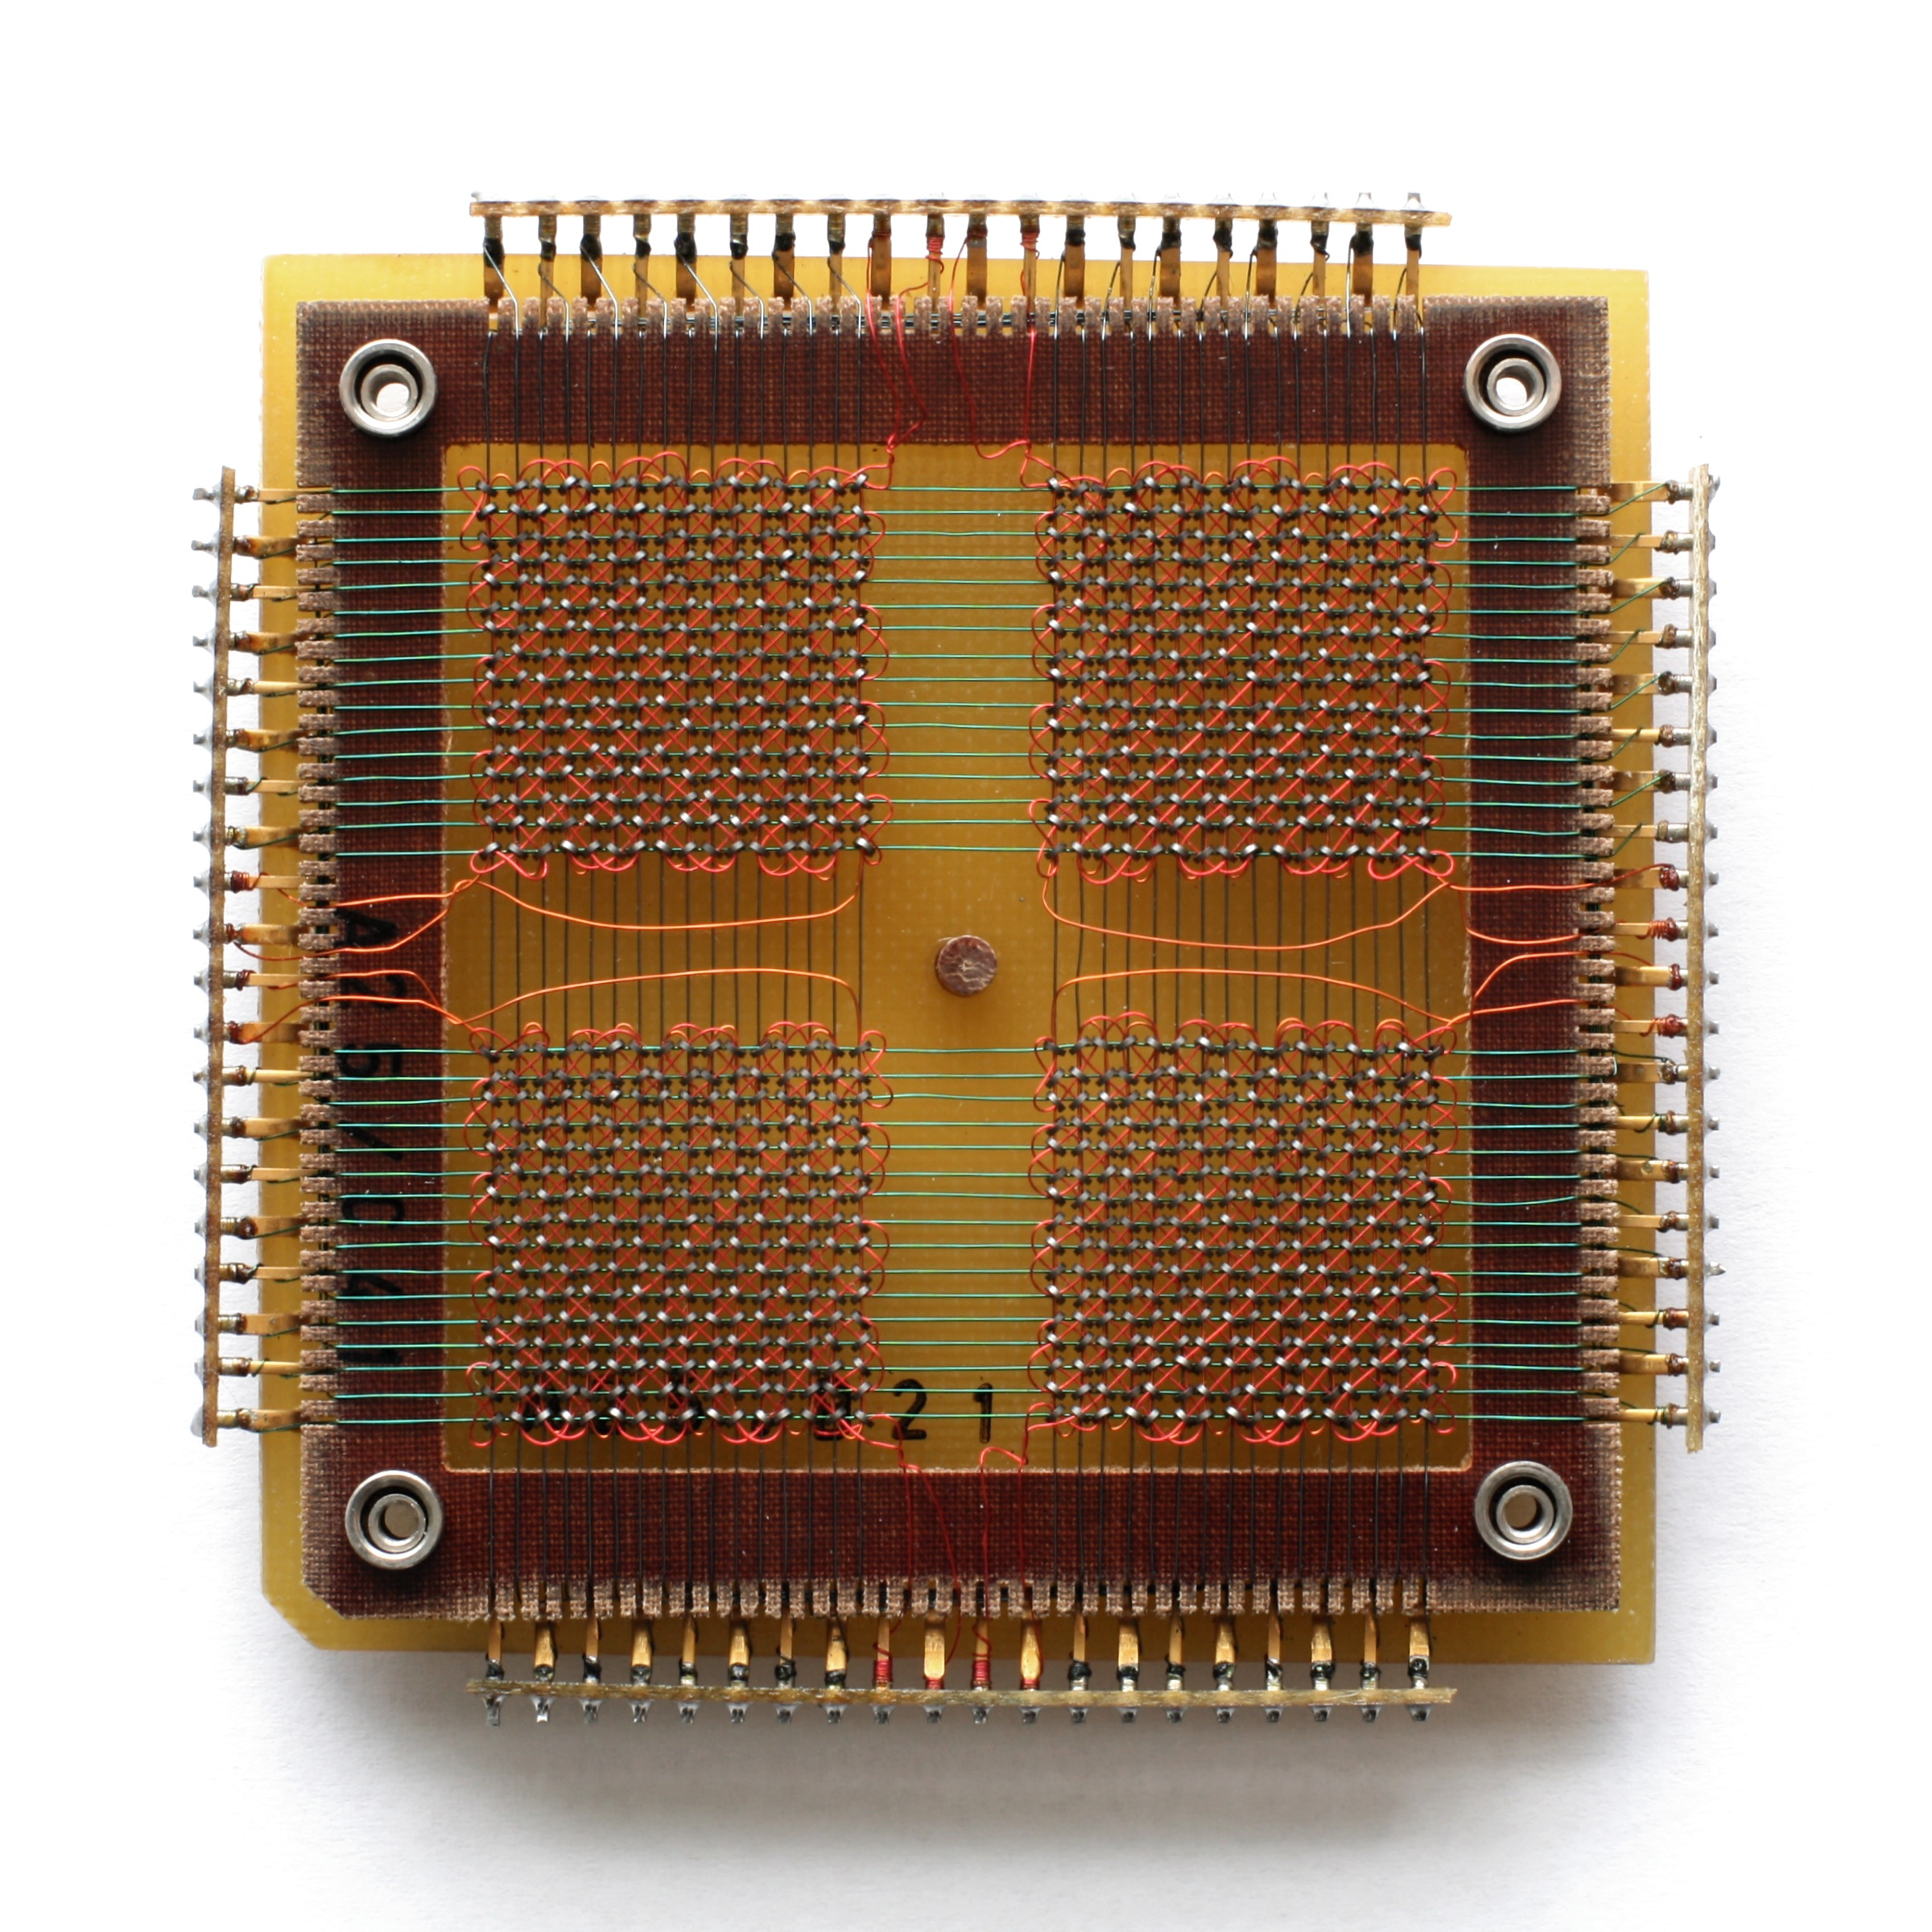
\includegraphics[width=0.35\textwidth]{figures/memory.jpg}
	\caption{\tiny This 32x32 core memory plane stores 1024 bits of information}
\end{figure}
\end{frame}

\begin{frame}
\frametitle{RAM}
\begin{itemize}
\item The RAM consists of multiple memory cells.
\item Each memory cell is uniquely identified by its memory address.
\item The first memory address always starts at 0, the last memory address depends on the amount of memory installed.
\end{itemize}

\begin{figure}
\center
\includegraphics[width=0.35\textwidth]{figures/RAM.jpg}
\caption{\tiny Example of writable volatile random-access memory}
\end{figure}
\end{frame}

\begin{frame}
\frametitle{Central Processing Unit}
\begin{itemize}
\item The RAM memory is under control of the CPU
\item The CPU can store a value in a specific memory cell in the RAM
\item The CPU can recall the stored value when prompted.
\end{itemize}
\begin{figure}
\center
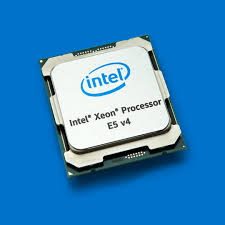
\includegraphics[width=0.35\textwidth]{figures/chip.jpg}
\end{figure}
\end{frame}

\section{The Unix operating system}

\begin{frame}
\frametitle{What is Unix?}
The Unix operating system is a set of programs that allow the user to communicate with the computer. \\~\

\end{frame}

\begin{frame}
\frametitle{What is Unix?}
The Unix operating system is a set of programs that allow the user to communicate with the computer. \\~\

The computer programs that allocate the system resources and coordinate all the details of the computer's internals is called the operating system or the kernel. \\~\
\end{frame}

\begin{frame}
\frametitle{What is Unix?}
The Unix operating system is a set of programs that allow the user to communicate with the computer. \\~\

The computer programs that allocate the system the system resources and coordinate all the details of the computer's internals is called the operating system or the kernel. \\~\

Users communicate with the kernel through a program known as the shell. The shell is a command line interpreter; it translates commands entered by the user and converts them into a language that is understood by the kernel. \\~\
\end{frame}


\begin{frame}
\frametitle{Unix framework}
The main concept that unites all the versions of Unix is the following four basics: \\~\

\begin{minipage}{.45\textwidth}
\textbf{1. Kernel:} The kernel is the heart of the operating system. It interacts with the hardware and most of the tasks like memory management, task scheduling and file management. 
\end{minipage} 
\begin{minipage}{.5\textwidth}
	
	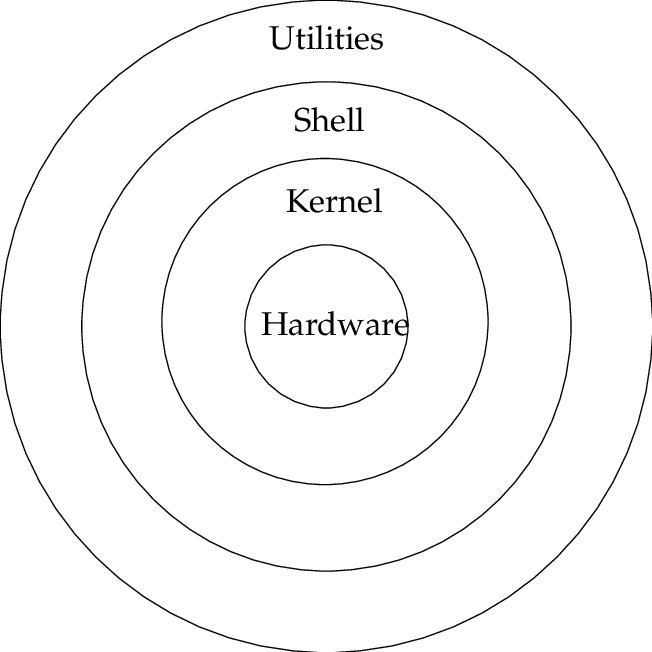
\includegraphics[width=0.8\textwidth]{figures/unix.png}
\end{minipage} 
\end{frame}

\begin{frame}
\frametitle{Unix framework}
The main concept that unites all the versions of Unix is the following four basics: \\~\

\begin{minipage}{.45\textwidth}
	\textbf{2. Shell:} The shell is the utility that processes your requests. When you type in a command at your terminal, the shell interprets the command and calls the program that you want. The shell uses standard syntax for all commands.
\end{minipage} 
\begin{minipage}{.5\textwidth}
	
	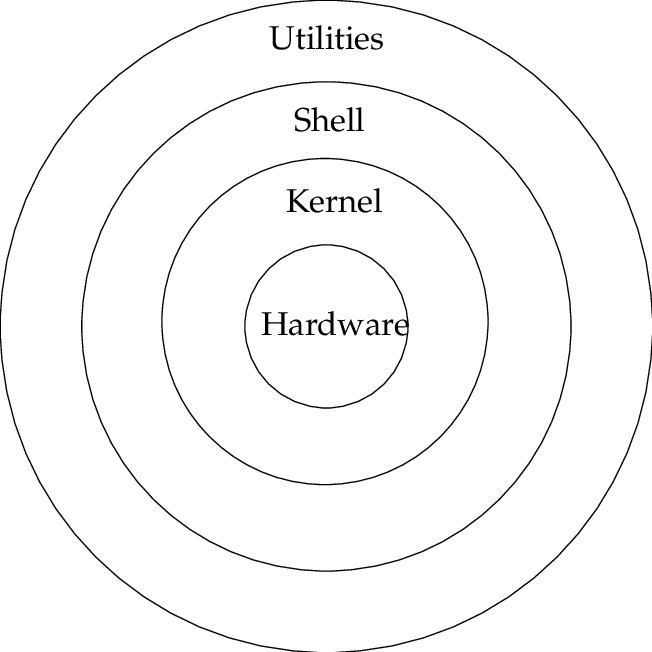
\includegraphics[width=0.8\textwidth]{figures/unix.png}
\end{minipage} 
\end{frame}

\begin{frame}
\frametitle{Unix framework}
The main concept that unites all the versions of Unix is the following four basics: \\~\

\begin{minipage}{.45\textwidth}
	\textbf{3. Commands and Utilities:} There are various commands and utilities which you can make use of in your day to day activities. \textbf{cp}, \textbf{mv}, \textbf{cat} and \textbf{grep}, etc. are few examples of commands and utilities. There are over 250 standard commands plus numerous others provided through 3rd party software. All the commands come along with various options.
\end{minipage} 
\begin{minipage}{.5\textwidth}
	
	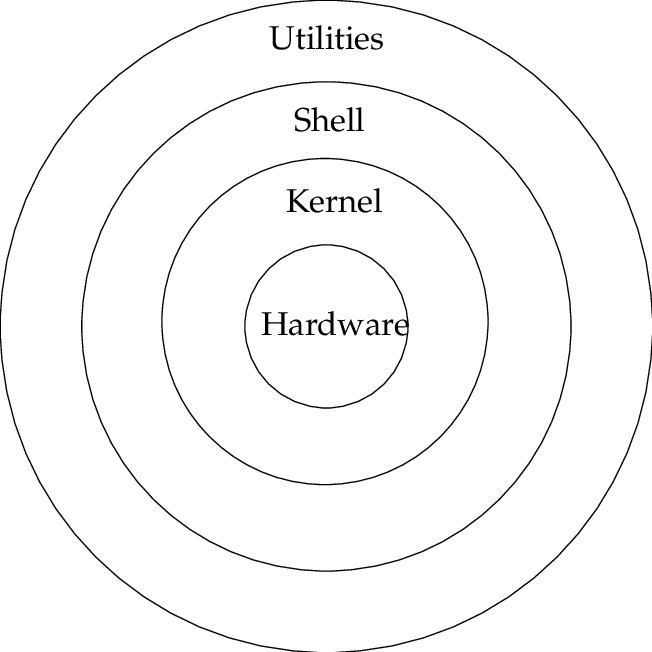
\includegraphics[width=0.8\textwidth]{figures/unix.png}
\end{minipage} 
\end{frame}

\begin{frame}
\frametitle{Unix framework}
The main concept that unites all the versions of Unix is the following four basics: \\~\

\textbf{4. Files and Directories} All the data of Unix is organized into files. All files are then organized into directories. These directories are further organized into a tree-like structure called the filesystem. 

\begin{figure}
	\centering
	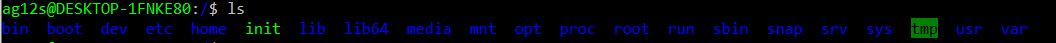
\includegraphics[width=\textwidth]{figures/files.jpg}
\end{figure}

\end{frame}

\section{Setting up the Bash Shell on Windows}
\begin{frame}
\frametitle{Setting up the Bash Shell on Windows}

1. Navigate to settings.
\begin{figure}
	\centering
	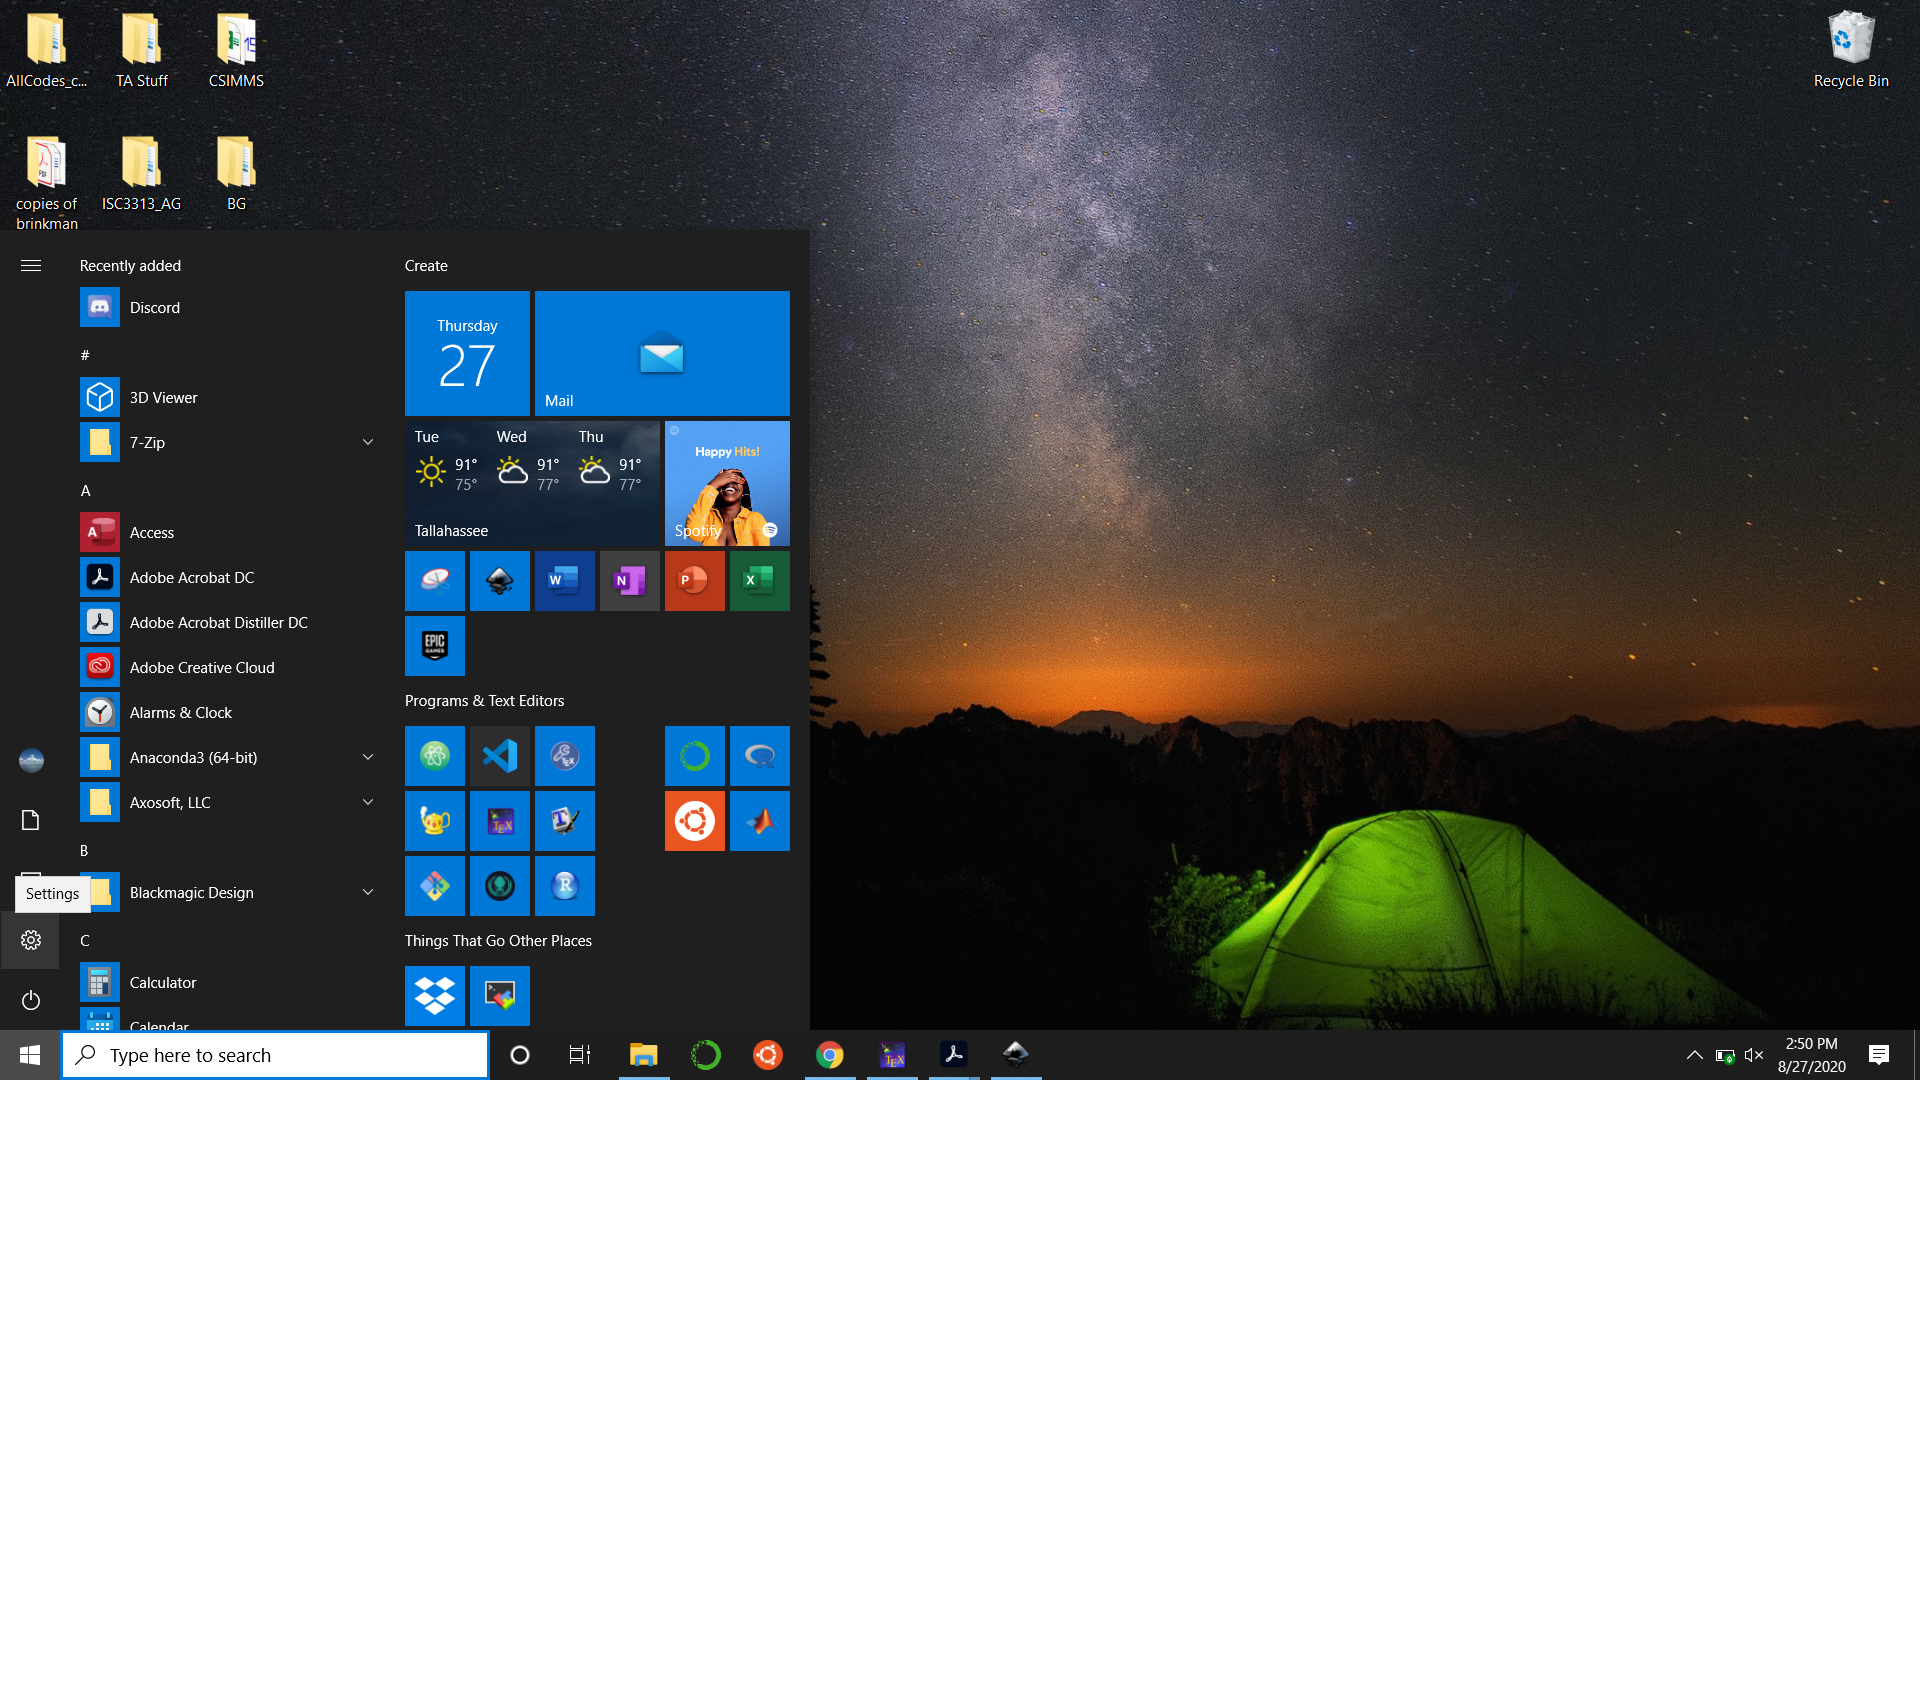
\includegraphics[width=\textwidth]{figures/step1.png}
\end{figure}
\end{frame}

\begin{frame}
\frametitle{Setting up the Bash Shell on Windows}
2. Click "Update and Security"
\begin{figure}
	\centering
	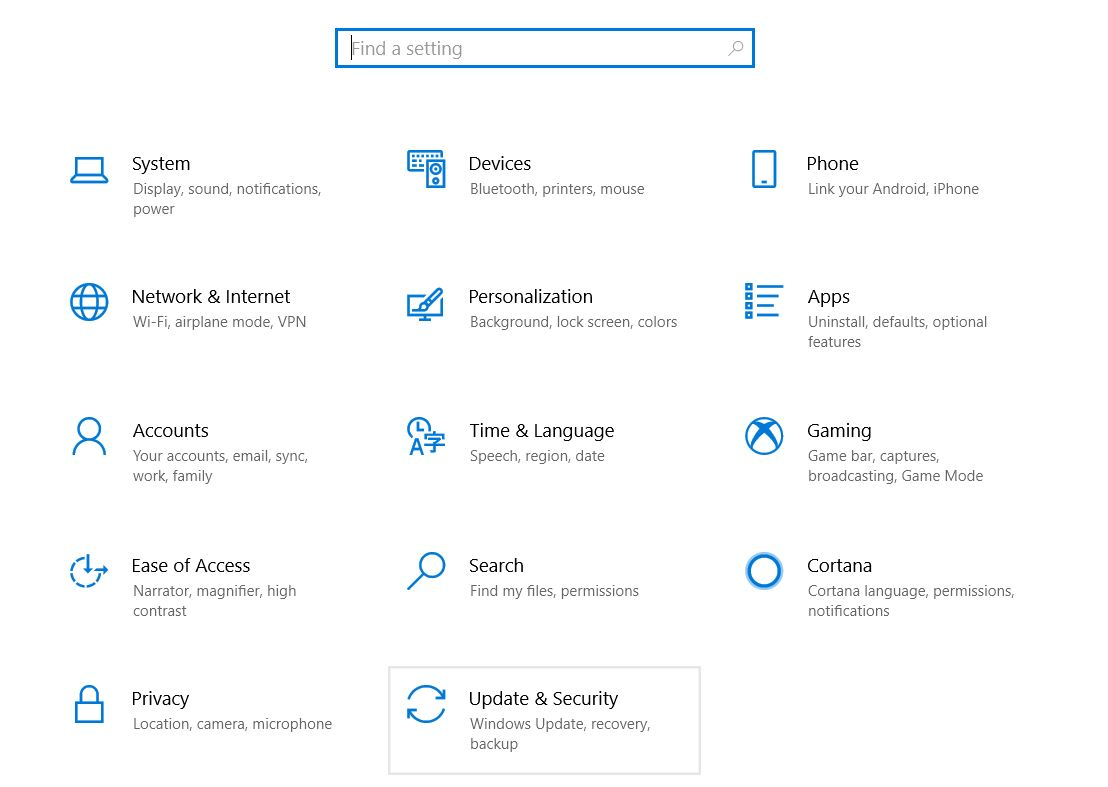
\includegraphics[width=.75\textwidth]{figures/step2.jpg}
\end{figure}
\end{frame}

\begin{frame}
\frametitle{Setting up the Bash Shell on Windows}
3. Select "For Developers" in the left column.
\begin{figure}
	\flushleft
	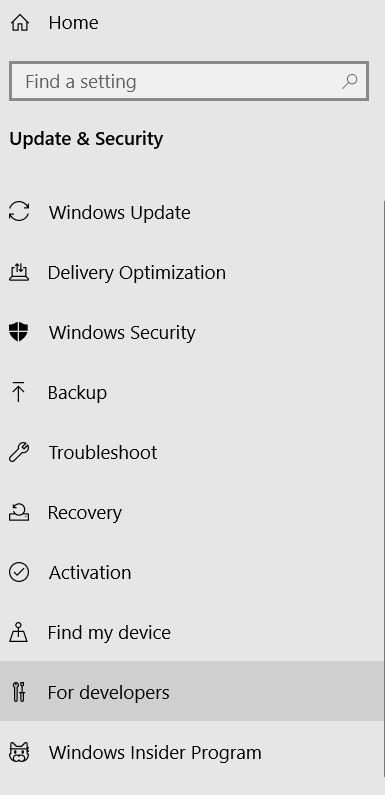
\includegraphics[width=0.35\textwidth]{figures/step3.jpg}
\end{figure}
\end{frame}

\begin{frame}
\frametitle{Setting up the Bash Shell on Windows}
4. Select "Developer Mode"
\begin{figure}
	\centering
	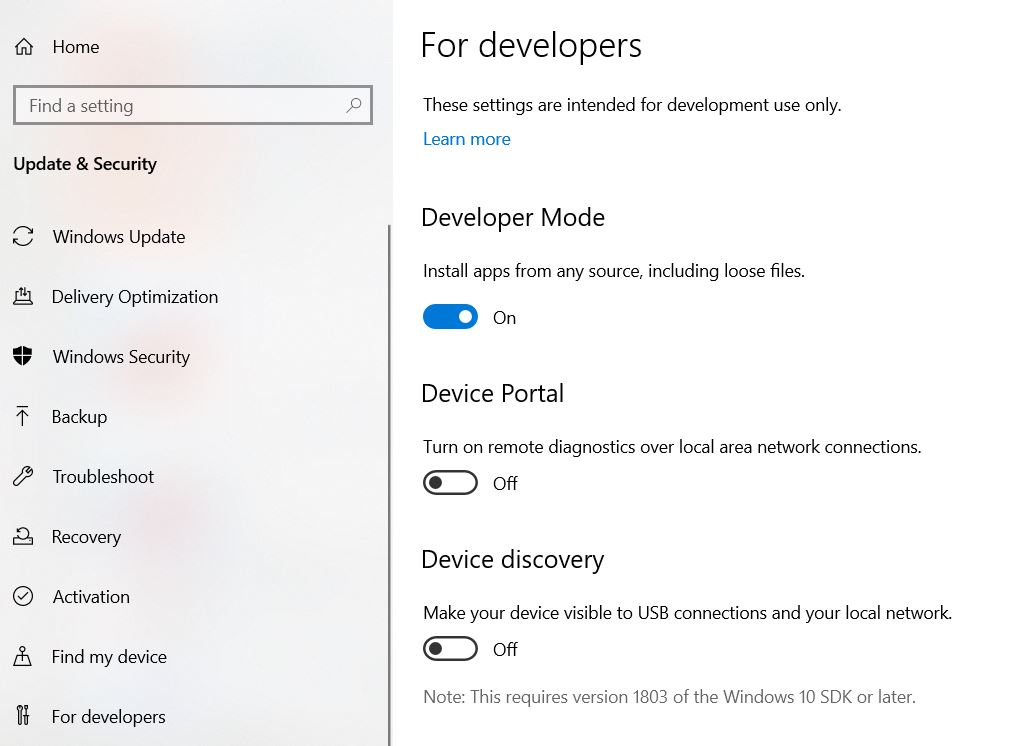
\includegraphics[width=0.65\textwidth]{figures/step4.jpg}
\end{figure}
\end{frame}

\begin{frame}
\frametitle{Setting up the Bash Shell on Windows}
5. Go to your control panel, select "Programs and Features"
\begin{figure}
	\centering
	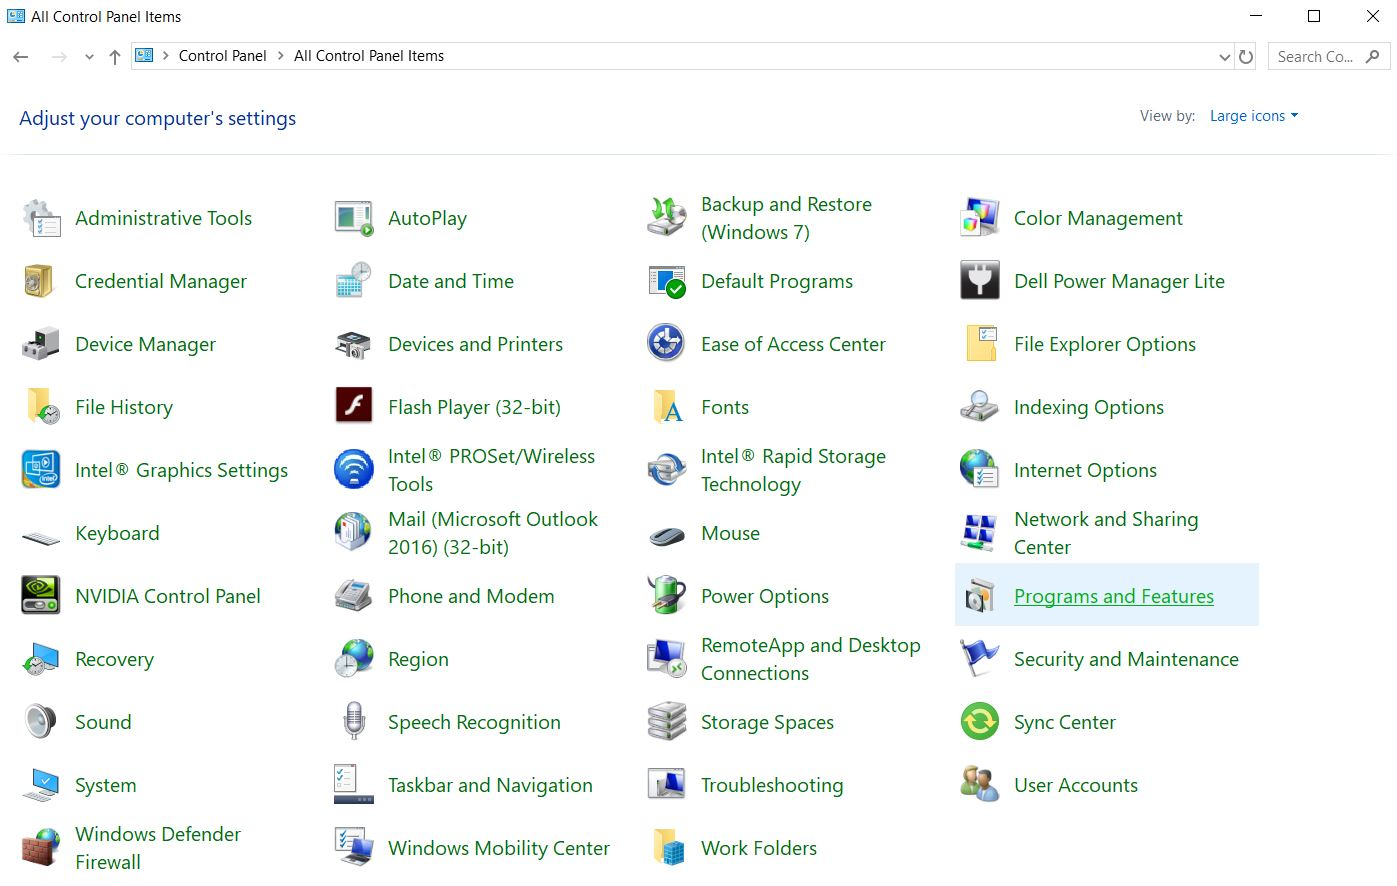
\includegraphics[width=0.7\textwidth]{figures/step5.jpg}
\end{figure}
\end{frame}

\begin{frame}
\frametitle{Setting up the Bash Shell on Windows}
6. Click "Turn Window's Features On or Off"
\begin{figure}
	\centering
	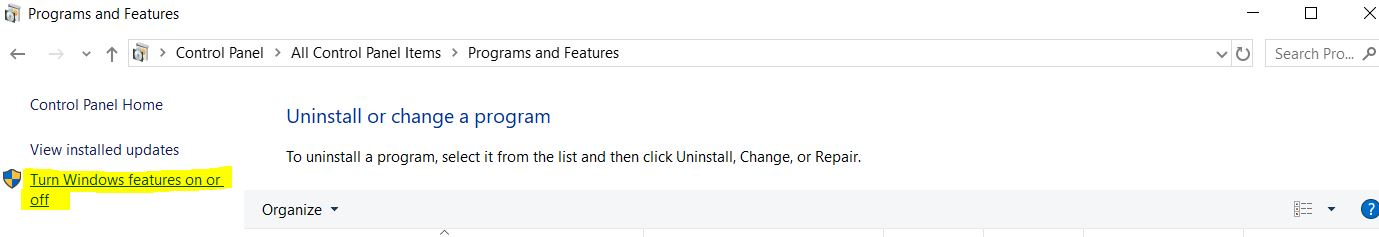
\includegraphics[width=0.7\textwidth]{figures/step6.jpg}
\end{figure}
7. Check the box next to "Windows Subsystem for Linux
\begin{figure}
	\centering
	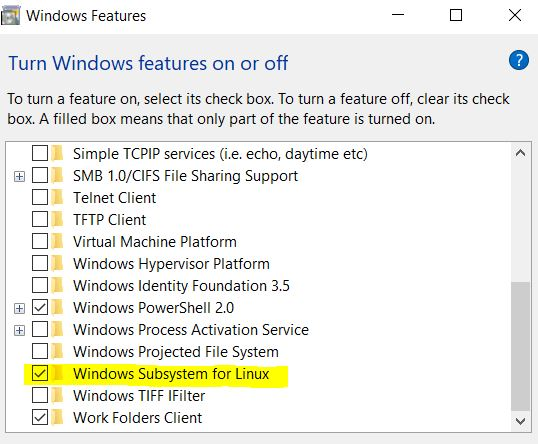
\includegraphics[width=0.5\textwidth]{figures/step7.jpg}
\end{figure}
8. Restart your computer.
\end{frame}

\begin{frame}
\frametitle{Setting up the Bash Shell on Windows}

9. Now that your computer has booted back up, search "Bash" in the search box and select the Run command.
\begin{figure}
	\centering
	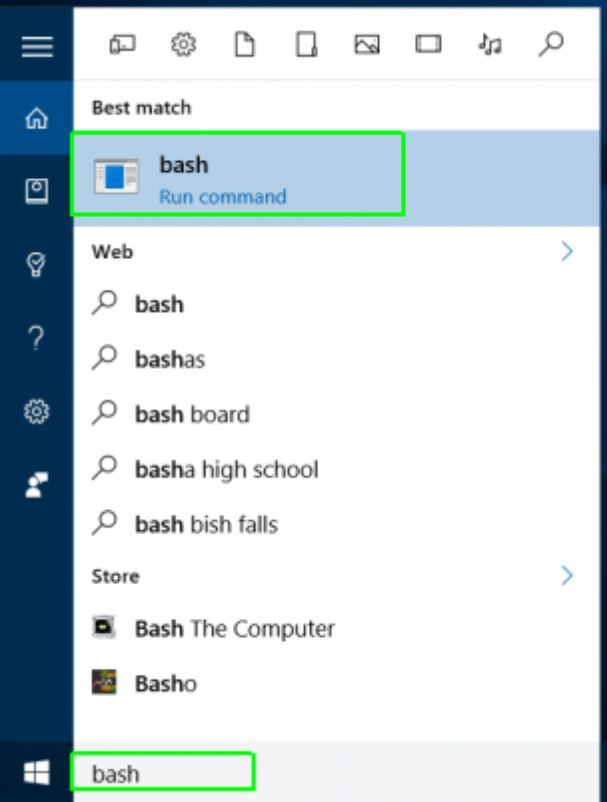
\includegraphics[width=0.35\textwidth]{figures/step8.jpg}
\end{figure}

10. Type "y" and hit Enter when promoted to install Ubuntu. The system will then take a few minutes to install Ubuntu in the command prompt window. \\~\

11. Create a username and password when prompted. NOTE: You will NOT see anything being typed for your password, but it is typing. 
\end{frame}

\begin{frame}
\frametitle{Starting Your Shell in Your User File}

\begin{enumerate}
   \item Open the Bash shell
   \item Type "cd \textasciitilde". This will bring you to the home directory.
   \item Type "vim .bashrc". This will open up a scary looking code in vim.
   \item Hit the down arrow until you make it to the bottom of this code.
   \item Type i - this is the short key for insert.
   \item Make a new line, and on the new line type "cd /mnt/c/Users/YOURUSERNAME"
   \item Hit the esc key
   \item Type ":wq"
   \item Restart Bash 
\end{enumerate}
I have mine set up to start on my Desktop. 
\begin{figure}
	\centering
	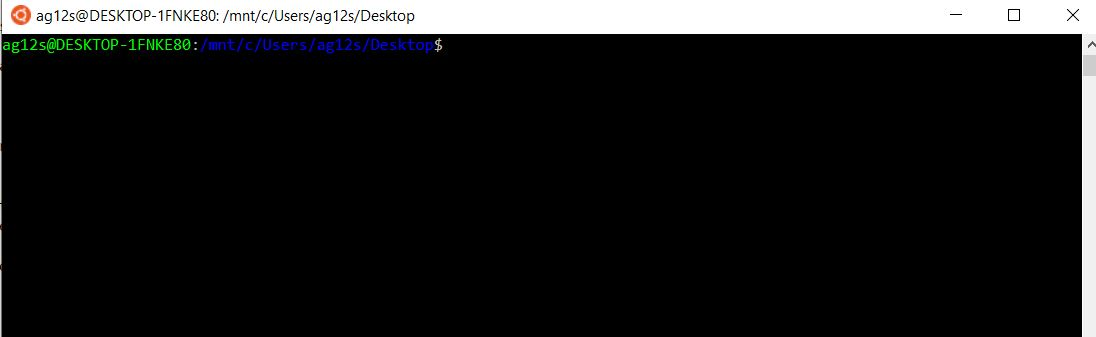
\includegraphics[width=0.85\textwidth]{figures/homeish.jpg}
\end{figure}
\end{frame}

\end{document}
